\documentclass[12pt,titlepage]{article}

% \usepackages21{fancyhdr}

\usepackage[printwatermark]{xwatermark}

\usepackage{grffile}
\usepackage{xcolor}
\usepackage{lipsum}
\usepackage{times}
\usepackage{soul}
\usepackage{epsfig}
\usepackage{rotating}
\usepackage{url}
\usepackage{latexsym}
\usepackage{graphicx}
\usepackage{amsfonts}
\usepackage{amsmath, amsthm, amssymb}
\usepackage{fullpage}
\usepackage{setspace}
\usepackage{natbib}
\usepackage{longtable}
\usepackage{keyval}
\usepackage{caption,subcaption}
\usepackage{arydshln}
%%\usepackage[hyphenbreaks]{breakurl}

%% allow urls to get broken on hyphens
\usepackage{hyperref}
\def\UrlBreaks{\do\/\do-}


%% APSR submission: no commas in citations between name and year
%% See http://merkel.zoneo.net/Latex/natbib.php
\bibpunct{(}{)}{;}{author-year}{}{;}

% the opening bracket symbol, default = (
% the closing bracket symbol, default = )
% the punctuation between multiple citations, default = ;
% the letter `n' for numerical style, or `s' for numerical superscript style, any other letter for author-year, default = author-year;
% the punctuation that comes between the author names and the year
% the punctuation that comes between years or numbers when common author lists are suppressed (default = ,);

\usepackage{footmisc}
\renewcommand{\footnotelayout}{\doublespacing} % set spacing in footnotes
\newlength{\myfootnotesep}
\setlength{\myfootnotesep}{\baselineskip}
\addtolength{\myfootnotesep}{-\footnotesep}
\setlength{\footnotesep}{\myfootnotesep} % set spacing between footnotes

% make footnote font size same as regular font size in text
\renewcommand{\footnotesize}{\normalsize} 


%% Use this for a "DRAFT" watermark
%% \newwatermark[allpages,color=pink!50,angle=45,scale=5,xpos=-25,ypos=40]{DRAFT}

%% List all locations for graphics here
\graphicspath{ {../plots/} }


\begin{document}
\sloppy
\thispagestyle{empty}

%% APSR submission requires double-spaced footnotes
%%\newcommand{\footnote}[1]{\footnote{\doublespacing #1}} %% <-- note \doublespacing here.

\renewcommand{\topfraction}{.85}
\renewcommand{\bottomfraction}{.7}
\renewcommand{\textfraction}{.15}
\renewcommand{\floatpagefraction}{.66}
\renewcommand{\dbltopfraction}{.66}
\renewcommand{\dblfloatpagefraction}{.66}

\newcommand{\yi}{\ensuremath{Y_i}}

% \urldef\myurlncsl1\url{foo%.com}
% \begin{document}
% text\footnote{WWW: \myurl}


\title{\Large{All in the family:\\Anna and Lisa Hahner's finishing
    times in\\the 2016 women's Olympic
  marathon}}\author{David Cottrell\thanks{Postdoctoral Research
  Fellow, Program in Quantitative Social Science, Dartmouth College,
    6108 Silsby Hall, Hanover, NH
    03755 (\texttt{david.cottrell@dartmouth.edu}).} \and Michael C.\
  Herron\thanks{Visiting Scholar, Hertie School of Governance, Berlin,
    Germany, and Professor of Government, Dartmouth College, 6108
    Silsby Hall, Hanover, NH 03755
    (\texttt{michael.c.herron@dartmouth.edu}).}}


\maketitle \doublespacing 

%\begin{abstract} 
% \noindent
%The abstract
%\end{abstract}

%\newpage


\begin{quote}
 \emph{``I invested all I had and 300 meters before the finish line, I was next to Lisa. It was a magical moment that we could finish this marathon together. We did not think about what we were doing.''�� - Anna Hahner} 
\end{quote}


\section*{Introduction}

On August 14, 2016, at 9:30 in the morning, the Women's Olympic
marathon kicked off in Rio de Janeiro, Brazil, when 156 runners from
80 countries across the world took off from the starting line en route
to their destination 42.195 kilometers away. Two hours, twenty-four
minutes, and four seconds later, Jemima Sumgong of Kenya would be the
first to cross the finishline and take home gold; Sumgong was just 3.5
minutes behind her personal best time in the marathon. Approximately
21 minutes later, twin marathoners from Germany, Anna and Lisa Hahner,
would cross the finishline together, holding hands and celebrating a
personal victory. Although the Hahners would finish 81st and 82nd,
respectively, with times slightly more than 18 minutes slower than
corresponding personal bests, Anna Hahner would describe their joint
finish as a ``magical moment.''
\href{https://www.nytimes.com/2016/08/17/sports/olympics/twins-finish-marathon-hand-in-hand-but-their-country-says-they-crossed-a-line.html}
The media quickly picked up on the Hanher story as an image of the
beaming twins finishing hand-in-hand captured a public audience. Many
believed the moment was a reflection of the Olympic spirit.

Not everyone agreed with this rosy interpretation. The twins' happy
facial expressions at the finish were portrayed as a bit contrived
(smiling like ``Honigkuchenpferde''---a Honigkuchenpferd is a German
cookie in the shape of a horse), and the sports director of the German
Athletics Federation, Thomas Kurschilgen, stirred up controversy when
he suggested that the Hahners' photo-finish was no coincidence.
Kurschilgen averred that the twins slowed down so as to finish
simultaneously and sought to create a spectacle and ``generate media
attention.'' Kurschilgen justified his charge with the fact that the
twins were at least 18 minutes behind their personal best
times.\footnote{\url{https://www.nytimes.com/2016/08/17/sports/olympics/twins-finish-marathon-hand-in-hand-but-their-country-says-they-crossed-a-line.html}}
Not surprisingly, these accusations were denied by the Hahners, who
claimed that their simultaneous finish was simply an unintended
coincidence.

%% Honigkuchenpferd quote from here:
%%
%% https://www.welt.de/sport/olympia/article157669264/Das-falsche-Laecheln-der-deutschen-Lauf-Zwillinge.html


What happened in the women's Olympic marathon, and how might we assess
whether the Hahner finish was coincidental or intentional? These two
interpretations are clearly at odds. If the former, then the Hahner
twins are to be celebrated and their finish treated as an expression
of the spirit behind the Olympic games. If the latter, though, then
the Hahner twins may have violated this spirt by not trying hard
enough. It is perhaps too easy for us to write such a glib
sentence---neither of us cannot fathom being able to complete a
marathon anywhere in the vicinity of two and a half hours---but we
nonetheless want to know what the data from the Olympic marathon data
tell us. Was the women's Olympic marathon a lovely coincidence or
something else?

Among female Olympic marathoners, the Hahner twins were not alone in
their familial ties, and we draw on this in the analysis that follows.
The marathon also featured twins from North Korea, Kim Hye-song and
Kim Hye-gyong, who had identical times and finished 10th and 11th,
respectively. The Kim finish, unlike the Hahner finish, appears devoid
of post-race controversy. Moreover, three triplets from Estonia
competed in the Rio marathon, although only two, Lily Luik and Leila
Luik, finished it, in 97th and 114th place, respectively. The third
Estonia triplet, Liina Luik, recorded what is known as a DNF---an
abbreviation that means did not finish, a term that we will use
throughout this article.

\section*{Marathon data}

For each participant who started the women's Olympic marathon, we know
several things: personal best marathon time prior to the 2016 Olympic
games; split times from the Rio marathon course at 5 kilometers, 10
kilometers, and so forth; and, finishing time. We cannot directly
observe the effort that an individual put into the race, and we do not
know why some runners have DNF results; some runners may have injured
themselves on the course and accordingly dropped out, and others may
have dropped out, uninjured, in anticipation of an unsatisfactory
result. Of the 156 marathon starters, 133 completed the race and 23
DNFed at various locations throughout the course. The overall DNF rate
was thus $\frac{23}{156} \approx 0.15$, and the relatively small
sample size at our disposal---156 runners---means that a 95\%
confidence for this rate is fairly wide, namely,
$\left(0.098, 0.22\right)$.

Key in the analysis that follows is the deviation between a runner's
Rio time and her prior personal best time in the marathon. Of course
there is variance across runners in these deviations, and we want to
know if patterns in the deviations support an honest effort by the
Hanher twins or perhaps something else.

\section*{The probability of an unintentional simultaneous finish}

Thomas Kurschilgen's accusations of an intentional finish stems from
two observations. First, the Hahner twins finished slower than he
expected, as we already noted recording times more than 18 minutes
slower than respective personal bests. Second, the twins finished
together at the exactly same time. Kurschilgen clearly believed that
neither of these events would have occurred had both Hahner run the
marathon independently, absent coordination. By his logic, the German
twins should have run faster and not have finished simultaneously.

On the other hand, only a handful of runners completed the Rio
marathon with times that were faster than their recorded best times.
Thus, 18 minutes behind a personal record may not be the outlier that
Kurschilgen claimed it to be. Moreover, there is good reason to
suspect that an unintended simultaneous finish was more likely for the
Hahner twin than it would be for any other set of runners. After all,
these two women are twins with presumably similar abilities. Not only
do they train together, but their pre-Rio best times are less than two
minutes apart. While Anna may be slightly faster than Lisa, measured
by personal bests, we might expect the difference in their Rio result
to be just as close as the differences in their recorded bests. And
given random variation in finishing times, a simultaneous finish might
not be out of the ordinary.

Even though they seem similar, finishing at very similar times and
finishing together are different phenomena. If, for example, both
Hahners were of similar ability to each other and also to many other
runners, then we might expect similar finishing times yet not
necessarily similar placements. The latter will be a function of the
extent to which all runners on the Rio course have similar talent
levels.  This point is an important one and will be evident in the
results that follow.

To test the assertion that the Hahner twins paced themselves to finish
at the same time and with back-to-back placements, we simply need to
compute the probability that such a result would have occurred
unintentionally. Hence we need to know the probability distribution of
Anna and Lisa's finishing times if their runs had been independent of
each other. The challenge, of course, is that this distribution is
unknown.  ^^ Therefore it needs to be estimated.

\section*{Modeling}

%% THIS SECTION IS A MESS.  I JUST WANTED TO PUT SOMETHING IN WRITING.

%% Ok.  Not sure what all the notation means.

% We know that Anna and Lisa Hahner finished the marathon in Rio
% simultaneously. We don't know, however, if the finish was intentional;

Suppose that Hahner the twins acted independently $I$ or they acted in
coordination $C$; these are the two possible states of the race
$\psi = \{I, C\}$. Given that we observed Anna and Lisa's finishing
times, $Y_A = y_A$ and $Y_L = y_L$, we want to know the probability
that they ran independently, as they say they did. Hence, we are
looking to determine,  %% y_a versus Y_a.  Former realized?

$$P(\psi = I \mid y_A  \cap y_L )$$

However, to determine this, we need to have some understanding of a
likelihood function that specifies Rio finishing times. We want to
know the likelihood of Anna's and Lisa's final times given
independence $P(y_A \cap y_L \mid \psi = I )$. We can estimate this
function with a few assumptions. First, we assume that under
independence, any given runner's final time $Y_i$ is conditional on
his/her running ability plus noise. Specifically, we assume that the
$Y_i$ is a linear function of the runner's ability $X_i$ plus a
normally distributed error term $e_i \sim N(0, \sigma)$. Second, we
assume that every runner shares the same linear relationship - meaning
the slope and intercept remain constant across runners. Third, we
assume that the error term is drawn from a common distribution across
runners. Hence, luck and misfortune are drawn from the same
distribution. Therefore,

$$Y_i \sim N(\beta_0 + X_{i}\beta_1 + e_i, \sigma)$$

We also assume that a runner's ability $X_i$ can be measured precisely
by her best marathon performance leading up to the Olympics. 

%% Any measurement error must therefore be negligible.

If Anna and Lisa intentionally slowed down as a result of coordination
then we would likely observe $y_A > E(Y_A \mid \psi = I) $ and
$y_L > E(Y_L\mid \psi = I )$. In other words, the final times that
Anna and Lisa recorded in the race would be greater than we would
expect if they had run independently.

Moreover, if Anna and Lisa coordinated to finish simultaneously, then
the difference between the two sisters' final times would be less that
the expected difference had they run independently. Therefore, under a
coordinated finish we would expect
$\left|y_A - y_L\right| < E(\left|Y_A - Y_L\right| \mid \psi = I )$.

\section*{Did Anna and Lisa intentionally slow down?}

According to Kurschilgen, Anna and Lisa underperformed in the Rio marathon. He claimed that because their goal was to finish simultaneously rather than finish at their fastest pace, their times were slower than they otherwise would have been.  He claimed that the twins were simply trading speed for a photo-finish.

If this were the case, the function generating Anna and Lisa's final times would deviate from the function that generated everyone else's final times.  Given everyone else would draw their times from the independent distribution  $Y_i \sim N(\beta_0 + X_{i}\beta_1 + e, \sigma)$,  Anna and Lisa would draw from a distribution of times that are slower in expectation. Hence, they would lie well-above the line that links a runner's performance in Rio to their previous best performance.    

\begin{figure}[!ht]
  \caption{Relationship between Personal Best and Result  -- better label?}
  \label{fig:scatter}
  \begin{subfigure}{.5\textwidth}
    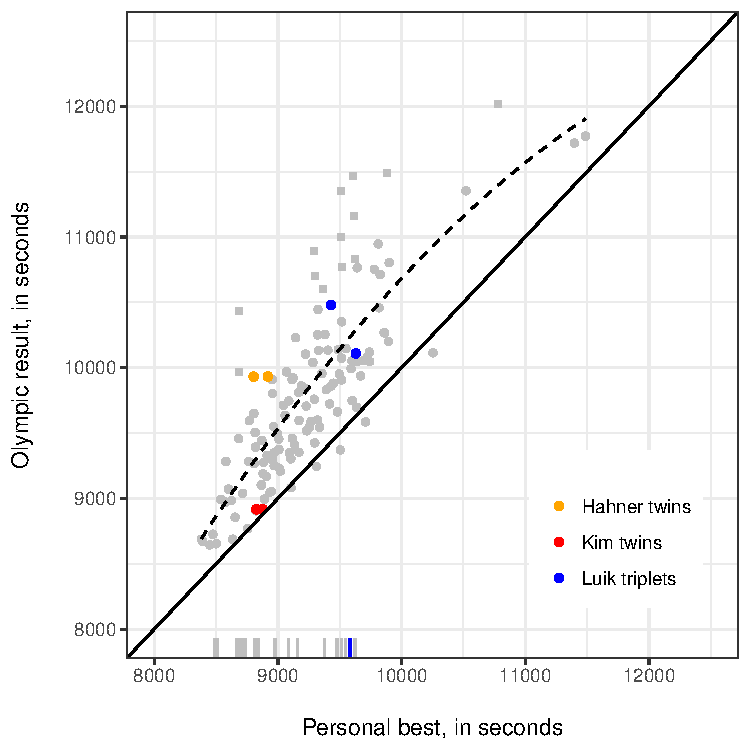
\includegraphics[width=\textwidth,
    keepaspectratio]{scatter_plot.pdf}
    \caption{Rio finishing times and personal best times}
    \label{fig:A}
  \end{subfigure}
  \begin{subfigure}{.5\textwidth}
    % \label{fig:Studentized Residuals}
    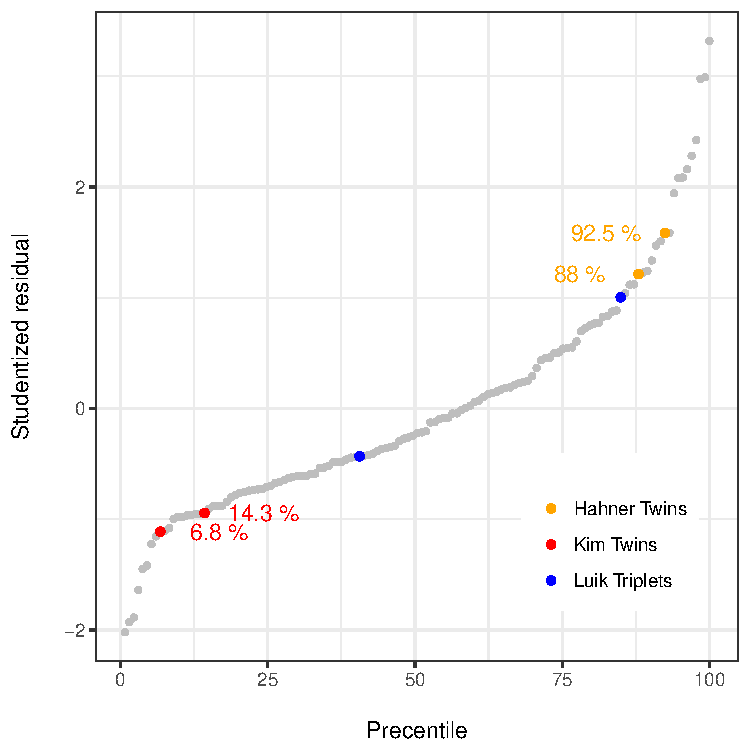
\includegraphics[width=.975\textwidth, keepaspectratio]{studentized_residuals.pdf}
    \caption{A}
    \label{fig:B}
  \end{subfigure}
\end{figure}

The scatter plot in Figure \ref{fig:scatter} displays the relationship between a runner's personal best and their final result.   Of the 156 runners that competed in the marathon event, 133 finished the race.  These individuals are plotted as grey points.  The 23 that did not finish are plotted below along the x-axis as grey tick-marks.   The dashed black line with grey confidence intervals represent OLS estimates of the linear relationship between the two variables.   The Hahner twins are marked by orange points. 

One can see that there is a clear linear relationship between a runner's performance in the olympics and her final result.  Moreover, there is a significant amount of noise in the relationship.  This suggests that despite one's innate abilities, luck plays a major role in olympic finishes.    Still, the twins' results are well above the fitted line, even accounting for typical error.  They are much slower than the underlying linear relationship suggests.  In fact, if we order each point by the size of the studentized residual (see the second plot), we can see that the Hahner twins are in the tail-end of the distribution.  Anna Hahner's residual deviation is greater than 91.7\% of the runners who completed the race while Lisa Hahner's deviation is greater than 86.5\%.  Hence, the twins appear to have finished at a much slower pace than expectation, which is what we might expect if they were coordinating their runs.\footnote{It is important to note that the North Korean twins finished much faster than expected.  XXXX explain PRK}   

\section*{Did Anna and Lisa intentionally finish together?}



\begin{figure}[!ht]
 \caption{Relationship between Difference in Personal Best and Difference in Result}
 \label{fig:diffdiff}
 \begin{subfigure}{.5\textwidth}
 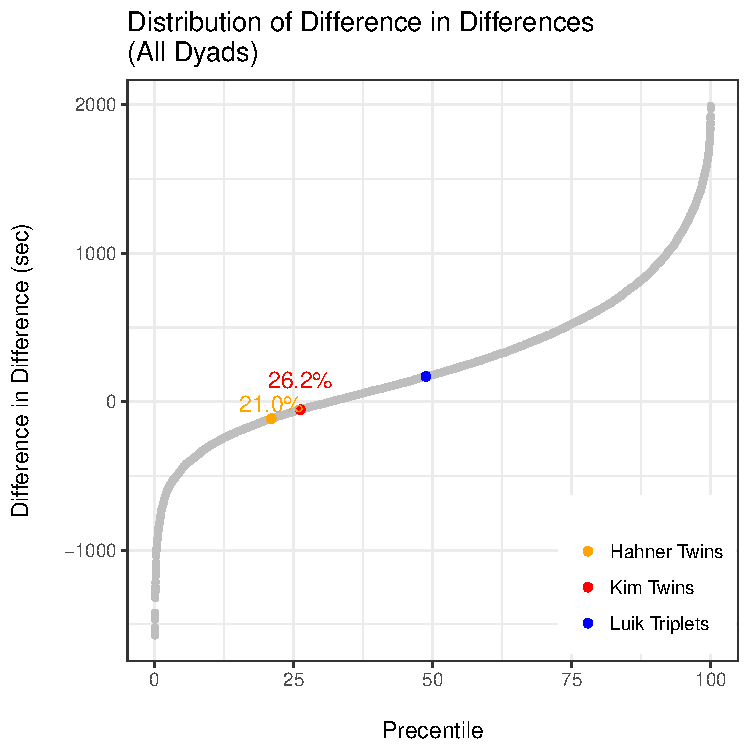
\includegraphics[width=\textwidth, keepaspectratio]{diff_in_diff_1.pdf}
 \end{subfigure}
 \begin{subfigure}{.5\textwidth}
 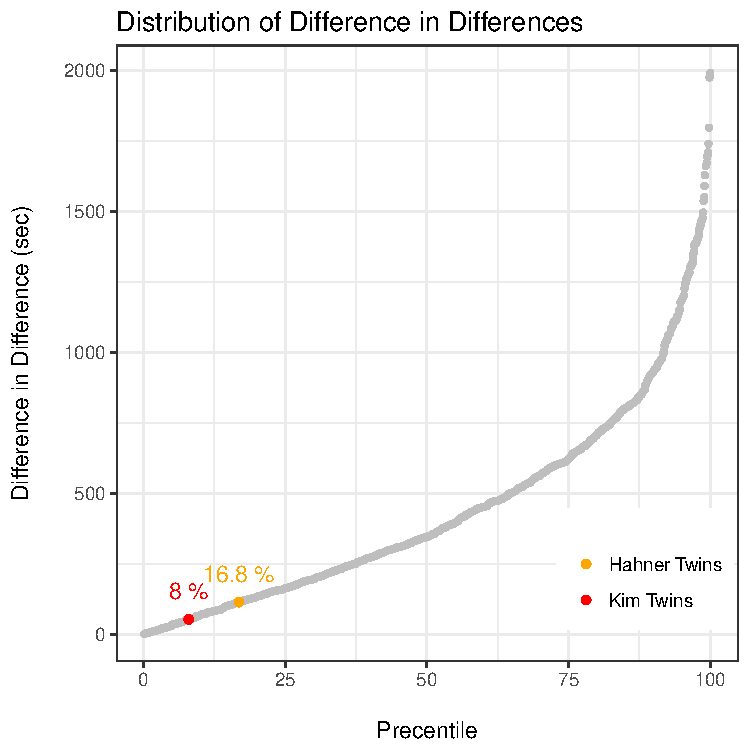
\includegraphics[width=\textwidth, keepaspectratio]{diff_in_diff_2.pdf}
 \end{subfigure}
\end{figure}

\newpage
\subsection*{Steps of the simulation}

\begin{enumerate}
\item Removing the twins from the sample, estimate a linear model that
predicts a runner?s final time ($Y_i$) based on her personal best time ($X_i$).
\item Extract the coefficients and the variance-covariance matrix from this
model.
\item For each runner, draw $\beta_0$ and $\beta_1$ from a multivariate normal
distribution with mean equal to the coefficients and variance equal to the
variance-covariance matrix.
\item For each runner, draw an error term ($e$) from a normal distribution with
mean equal to zero and a standard deviation equal to the standard
deviation of the model?s residuals ($\sigma$).
\item For each runner, predict the final result by combining the randomly
generated beta coefficients and error terms, $\hat{y} = \beta_0 + \beta_1 + e$.
\item Eliminate each runner from the race with a probability equal to the
percent of the total runners who did not finish in the actual race.  This
account for the likelihood of a DNF.
\item Calculate the difference in time between Anna Hahner and Lisa Hahner.
\item Calculate the difference in ranking between Anna Hahner and Lisa Hahner.
\item Repeat steps 3 through 8 ten thousand times.
\item Plot a histogram of the results in Figure \ref{fig:simdiff}
\end{enumerate}

\begin{figure}[!ht]
 \caption{The distribution of simulated results}
 \label{fig:simdiff}
 \begin{subfigure}{.5\textwidth}
 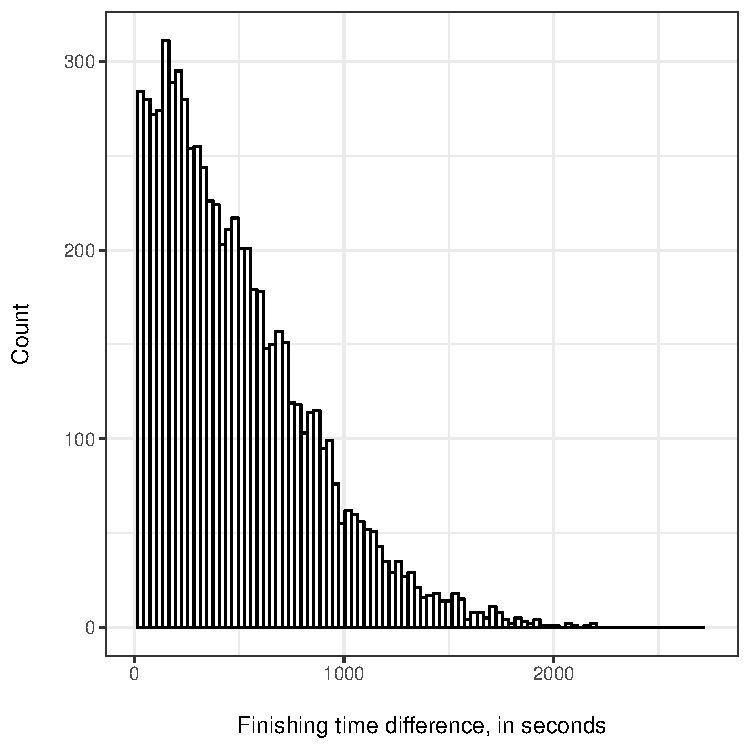
\includegraphics[width=\textwidth, keepaspectratio]{simulated_time.pdf}
 \end{subfigure}
 \begin{subfigure}{.5\textwidth}
 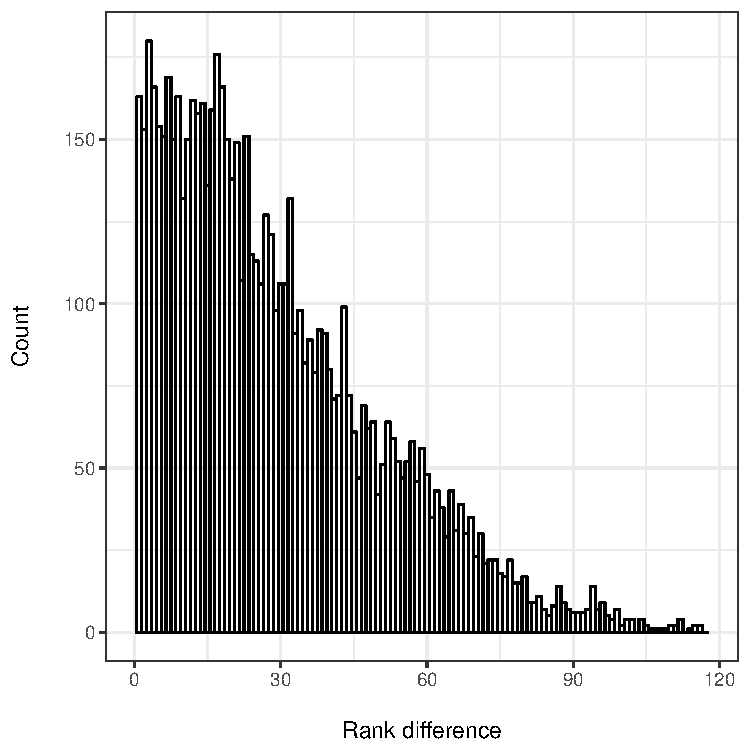
\includegraphics[width=\textwidth, keepaspectratio]{simulated_rank.pdf}
 \end{subfigure}
\end{figure}






   

\end{document}

